\chapter{Blutdruckmessung ohne und mit Stethoskop}
\section{Allgemein}
\begin{figure}[H]
    \centering
    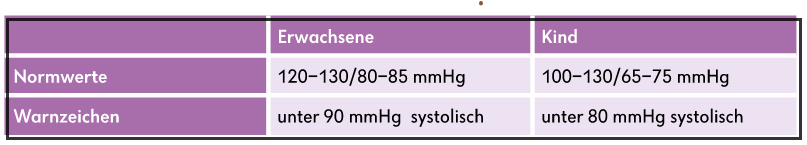
\includegraphics[width=\textwidth]{res/blutdruck.png}
\end{figure}

\section{Ohne Stethoskop - Palpatorisch}
\begin{enumerate}
    \item Manschette um Oberarm legen
    \item Stellschraube schließen, Puls am Arm tasten
    \item So lange aufpumpen, bis kein Puls mehr spürbar ist, dann 2x drücken
    \item Vorsichtig die Stellschraube öffnen, damit Luft langsam entweicht
    \item Sobald Puls wieder spürbar $\implies$ Systolischer Blutdruck
    \item Luft ganz auslassen
\end{enumerate}

\section{Mit Stethoskop - Auskulatorisch}
\begin{enumerate}
    \item Manschette um Oberarm legen
    \item Stellschraube schließen, Puls tasten
    \item So lange aufpumpen, bis kein Puls mehr spürbar ist, dann 2x drücken
    \item Stethoskop in der Ellenbeuge ansetzen
    \item Stellschraube öffnen
    \item Sobald pulsartige Geräusche hörbar sind $\implies$ Systolischer Blutdruck
    \item Geräusche hören auf $\implies$ Diastolischer Blutdruck
    \item Luft ganz auslassen
\end{enumerate}
